%%
%% Multi-Agent Large Language Model Pipeline for Cross-Domain Systematic
%% Literature Review Automation: A Five-Specialty Evaluation Across 62 RCTs
%%
%% AUTHOR VERSION. Acknowledgements remain blank until acceptance and any
%% funding disclosures are confirmed.
%%
\documentclass[a4paper,fleqn]{cas-sc}

\usepackage[authoryear,longnamesfirst]{natbib}
\usepackage{booktabs}
\usepackage{multirow}
\usepackage{array}
\usepackage{graphicx}
\usepackage{amsmath,amssymb}
\usepackage{hyperref}
\usepackage{lineno}

\begin{document}
\let\WriteBookmarks\relax
\def\floatpagepagefraction{1}
\def\textpagefraction{.001}

\shorttitle{Multi-Agent LLM Pipeline for Cross-Domain SLR}
\shortauthors{B. Gurram}

\title[mode = title]{Multi-Agent Large Language Model Pipeline for
Cross-Domain Systematic Literature Review Automation: A Five-Specialty
Evaluation Across 62 Randomized Controlled Trials}

\author[1]{Bhaskar Gurram}[orcid=0009-0005-2947-102X]
\cormark[1]
\ead{gurrambhaskar.ai@gmail.com}
\credit{Conceptualisation, Methodology, Software, Investigation, Data
curation, Formal analysis, Visualisation, Writing -- original draft,
Writing -- review \& editing}
\affiliation[1]{organization={ZASTI},
            country={India}}
\cortext[1]{Corresponding author}

\begin{abstract}
Systematic literature reviews (SLRs) are foundational to evidence-based
medicine but cost an estimated 1{,}000--2{,}000 person-hours each.
Large language models (LLMs) promise automation, yet most evaluations
target a single domain or model, leaving open how robust LLM extraction is
across specialties and across the closed/open-weights frontier. We built
an end-to-end multi-agent pipeline (retrieval, abstract screening,
full-text fetch, full-text eligibility, deduplication, 11-field structured
extraction) and ran it across five published SLRs covering pediatric
epilepsy, heart failure, advanced melanoma, treatment-resistant depression
and chronic obstructive pulmonary disease (62 ground-truth RCTs).
Four frontier LLMs were evaluated on extraction with a single locked
prompt: GPT-4o-mini, Llama 3.3 70B, Qwen 3 235B-A22B and DeepSeek V3.
Mean retrieval recall was 96.2\%, and end-to-end pipeline F1 ranged
from 0.30 (COPD) to 1.00 (epilepsy). Post-processed extraction accuracy
averaged 78.2\% across all 4 models and 5 reviews; the two open
mixture-of-experts models (Qwen 3 235B 80.9\%, DeepSeek V3 80.8\%)
outperformed both the closed baseline (GPT-4o-mini 75.9\%) and the dense
open model (Llama 3.3 70B 75.1\%). Crossover-trial recognition was a
clean model-quality signal (Qwen 5/6, DeepSeek 4/6, Llama 3/6, GPT 2/6).
Total extraction cost was USD 2.37, full-pipeline cost USD 3.21. Open
MoE models match or exceed closed baselines on structured medical
extraction at lower cost, and ground-truth framing decisions act as a
measurable evaluation confound that future SLR-automation benchmarks
should annotate.
\end{abstract}

\begin{highlights}
\item Multi-agent LLM pipeline tested on 5 medical specialties and 62 RCTs
\item Open mixture-of-experts models match or beat closed baselines on extraction
\item Mean v2 extraction accuracy 78.2\% across four frontier LLMs and five domains
\item Crossover trial recognition splits models: Qwen 5/6 vs GPT-4o-mini 2/6
\item Total cost USD 3.21 across all five reviews demonstrates production viability
\end{highlights}

\begin{keywords}
systematic literature review \sep large language models \sep
multi-agent systems \sep evidence synthesis \sep healthcare informatics \sep
cross-domain validation \sep mixture of experts
\end{keywords}

\maketitle

\linenumbers

% =============================================================================
\section{Introduction}\label{sec:intro}

Systematic literature reviews (SLRs) and meta-analyses are foundational
artefacts of evidence-based medicine and policy-making
\citep{higgins2019cochrane,page2021prisma}. They synthesise primary
evidence into reproducible, transparent assessments of intervention
effects, but their production is costly: empirical surveys based on the
PROSPERO registry report a median of 67 weeks and at least
two-reviewer effort to publication
\citep{borah2017slrtime,allen1999estimatingtime}. The growth in primary
trials has further widened the gap between evidence produced and evidence
synthesised: the often-cited estimate is that more than 75 trials and
11 systematic reviews are published each day, a rate that human
review teams cannot match without automation
\citep{bastian2010seventyfive,elliott2017living}.

Three generations of automation have responded to this pressure. The first
brought information-retrieval-style heuristics and supervised
classifiers for citation screening
\citep{cohen2006reducing,wallace2010active,bannach2019machine}. The second
embedded these classifiers into review platforms such as
EPPI-Reviewer~\citep{thomas2017eppi}, RobotReviewer~\citep{marshall2017robotreviewer},
ASReview~\citep{vandeschoot2021asreview} and SWIFT-Review~\citep{howard2016swift},
plus large-scale evidence-synthesis tools like
Rayyan~\citep{ouzzani2016rayyan} and the Covidence ecosystem analysed by
\citet{harrison2020covidence,vandinter2021distillersr}. The third, which
this paper addresses, applies large language models (LLMs) to screening,
full-text eligibility and structured data extraction
\citep{khraisha2024llmsr,gartlehner2024aisr,guo2024llmsr,wang2023llmscreen,
syriani2024screening,sundaram2023automating}.

The third generation has matured rapidly. \citet{khraisha2024llmsr}
benchmarked GPT-4 across screening and extraction in multilingual
literature and reported chance-corrected agreements that ranged from
``none'' to ``moderate''. \citet{gartlehner2024aisr} extracted nine
structured fields from 10 RCTs and observed model-dependent error patterns.
\citet{guo2024llmsr} compared GPT-3.5 and GPT-4 on automated paper
screening for clinical reviews. These studies share three limitations
that, taken together, motivated the present work. First, most evaluations
target a single clinical domain, so it is unclear whether reported
accuracies would generalise across specialties with different trial
designs and reporting conventions. Second, most evaluations test a
single closed-weights model (almost always GPT-4 family); the rapid
emergence of competitive open-weights mixture-of-experts (MoE) models
\citep{grattafiori2024llama3,yang2025qwen3,deepseekv3,shazeer2017moe}
has not been systematically benchmarked against closed baselines on SLR
extraction. Third, ground-truth construction itself encodes
review-specific analytical decisions that may penalise
extraction agents for reproducing the source paper's stated values
rather than the SLR authors' downstream re-coding; this confound is rarely
made explicit in published evaluations.

We address these gaps by building an end-to-end multi-agent SLR pipeline
and evaluating it across five completed and published systematic reviews
spanning pediatric neurology, cardiology, oncology, psychiatry and
respiratory medicine. The five reviews span 62 included randomised
controlled trials (RCTs) and four trial-design archetypes (parallel-group
fixed dose, parallel-group dose-comparison, multi-arm checkpoint inhibitor
combinations and crossover psychotropic infusions). All five reviews were
processed with a single locked extraction prompt and the same four LLMs:
GPT-4o-mini~\citep{achiam2023gpt4}, Llama 3.3 70B
Instruct~\citep{grattafiori2024llama3}, Qwen 3 235B-A22B~\citep{yang2025qwen3}
and DeepSeek V3~\citep{deepseekv3}.

The contributions of this paper are six-fold:

\begin{enumerate}
\item An end-to-end multi-agent SLR pipeline (six agents from PubMed retrieval
through structured extraction) that produces auditable outputs at every
stage and operates at a total cost below USD 4 per five-review batch.
\item The first cross-domain LLM extraction benchmark against five published
SLRs in five distinct medical specialties using a single locked schema and
prompt.
\item Head-to-head evaluation of two open-weights MoE models (Qwen 3 235B,
DeepSeek V3) against a strong closed baseline (GPT-4o-mini) and a strong
dense open model (Llama 3.3 70B); the open MoE models lead the ranking.
\item A four-finding inventory of \emph{cumulative cross-review patterns}:
GT-vs-source-paper framing tension, crossover-trial recognition, multi-arm
sample-size confusion specific to GPT-4o-mini, and domain-dependent field
difficulty.
\item A two-pass evaluation protocol (raw and ``v2'' post-processed) that
isolates LLM extraction failure from format-mapping failure on the
\texttt{first\_author} field, and quantifies the +7--9 percentage-point
accuracy gain achievable by injecting PubMed metadata.
\item A complete cost analysis and a public, fully reproducible release of
prompts, schema, ground truths, model outputs and evaluation scripts.
\end{enumerate}

The remainder of this paper is organised as follows. Section~\ref{sec:related}
surveys related work. Section~\ref{sec:methods} describes the pipeline,
the four models, the schema, the ground-truth construction protocol and
the evaluation procedure. Section~\ref{sec:results} reports
pipeline performance, extraction accuracy at the model and field level,
the four cross-review findings and a cost analysis.
Section~\ref{sec:discussion} compares with prior work and draws
methodological implications. Section~\ref{sec:limitations} documents
limitations, and Section~\ref{sec:conclusion} concludes.

% =============================================================================
\section{Related Work}\label{sec:related}

\subsection{Pre-LLM machine-learning approaches to SLR automation}

Citation screening was the first SLR sub-task to receive sustained
machine-learning attention. \citet{cohen2006reducing} demonstrated that a
support-vector classifier trained on review-specific decisions could
substantially reduce the screening workload while preserving sensitivity.
\citet{wallace2010active} introduced active-learning protocols that
prioritise borderline records for human review. \citet{howard2016swift}
released SWIFT-Review, a workbench combining topic models with iterative
classifier training. \citet{przybyla2018prioritising} extended the
paradigm with relevance feedback and showed work-saved-over-sampling
gains of 30--60\% across diverse review domains.
\citet{bannach2019machine} and \citet{marshall2019toward} reviewed the
field and highlighted that, despite robust empirical gains in single-review
benchmarks, transfer across reviews and across specialties remained
unsolved by classical methods.

\subsection{LLMs for screening}

The first LLM-based screening studies appeared in 2023.
\citet{wang2023llmscreen} examined whether GPT-4 could write
\emph{Boolean} search queries comparable to expert search-strategists.
\citet{syriani2024screening} reported precision and recall trade-offs
when ChatGPT was applied to title/abstract screening across review topics
and found models outperformed simple baselines but lagged
review-specific classifiers. \citet{guo2024llmsr} formalised the
methodology in JMIR and reported moderate agreement with human screeners on
clinical reviews. These studies establish that LLMs can act as competent
first-pass screeners but disagree on whether they should be deployed as
sole screeners.

\subsection{LLMs for full-text extraction}

Full-text extraction is the costliest SLR sub-task. \citet{gartlehner2024aisr}
extracted nine structured fields (population, intervention, outcomes
etc.) from 10 RCTs using Claude 2 and reported per-field accuracy
ranging from 76\% to 100\%, with population-related fields hardest.
\citet{whitton2025evidence} and \citet{thirunavukarasu2023llmmedicine}
reviewed the landscape of medical LLM applications and noted that
extraction accuracy is harder to evaluate than screening accuracy because
ground truth is a structured object rather than a binary label.
\citet{khraisha2024llmsr} ran the largest end-to-end study to date,
applying GPT-4 to multilingual peer-reviewed and grey literature; their
chance-corrected metrics suggested that data-extraction accuracy was
``moderate'' and that headline accuracies could be inflated by class
imbalance.

\subsection{Multi-LLM benchmarking efforts}

Few studies have systematically compared multiple LLMs on the same SLR
task. The HELM benchmark \citep{liang2023helm} and BIG-Bench
\citep{srivastava2023bigbench} enable cross-model comparison on general
language tasks, but neither targets SLR extraction. The medical-LLM
review of \citet{lee2024evaluation} and the surveys of
\citet{pressman2024clinicalllm,maity2025healthcare} highlight that 90\% of
published medical-LLM evaluations test only one or two closed models,
and that head-to-head open/closed comparisons in clinical extraction
remain rare.

\subsection{Cross-domain validation gaps}

The single most consistent gap in the prior literature is that nearly all
extraction studies fix a single review (or family of reviews on related
topics) and a single model. The structural variability that distinguishes
domains --- parallel-group monotherapy versus multi-arm dose comparison
versus crossover infusion --- is therefore not exercised by single-domain
benchmarks. Table~\ref{tbl:related} summarises the closest prior studies
and the dimensions on which the present work extends them.

\begin{table*}[t]
\caption{Summary of prior multi-LLM SLR studies and the dimensions on
which the present work extends them. Domains: number of independent
clinical specialties; Models: number of LLMs benchmarked; Trials:
ground-truth trials evaluated.}
\label{tbl:related}
\begin{tabular*}{\tblwidth}{@{}p{4.0cm}p{2.0cm}p{1.5cm}p{1.5cm}p{1.5cm}p{4.5cm}@{}}
\toprule
Study & Task & Domains & Models & Trials & Notes \\
\midrule
\citet{cohen2006reducing}    & Screening   & 15 & 0 (SVM) & ---  & Pre-LLM, supervised classifiers \\
\citet{wallace2010active}    & Screening   &  3 & 0       & ---  & Active learning \\
\citet{vandeschoot2021asreview} & Screening & many & 0 (rule) & --- & Open-source platform \\
\citet{wang2023llmscreen}    & Query gen.  &  4 & 1 (GPT-4) & --- & Boolean query construction \\
\citet{syriani2024screening}& Screening   &  3 & 1 (ChatGPT) & --- & Title/abstract \\
\citet{guo2024llmsr}         & Screening   &  3 & 2 (GPT-3.5/4) & --- & Clinical reviews \\
\citet{khraisha2024llmsr}    & Screen + extract & 2 & 1 (GPT-4) & --- & Multilingual \\
\citet{gartlehner2024aisr}   & Extraction  &  1 & 1 (Claude 2) & 10 & Nine-field schema \\
\textbf{This work}           & Full pipeline & \textbf{5} & \textbf{4} & \textbf{62} &
Closed and open MoE; locked prompt; cumulative findings \\
\bottomrule
\end{tabular*}
\end{table*}

% =============================================================================
\section{Methods}\label{sec:methods}

\subsection{Study design}

We designed a six-agent pipeline (Section~\ref{sec:methods:arch}) that
takes a PubMed query and a set of inclusion criteria as input and produces
structured extractions for the included primary RCTs as output. We then
ran the pipeline against five published SLRs whose source papers, search
strategies, inclusion criteria and full citation lists are public,
treating each SLR's published inclusion list as the ground truth.
Extractions were evaluated against an 11-field structured schema
(Section~\ref{sec:methods:schema}) for the subset of ground-truth trials
that survived the upstream pipeline stages.

\subsection{Source systematic reviews}

The five source SLRs were chosen to span diverse clinical specialties,
trial-design archetypes and publication ages, and to include a mix of
single-arm placebo-controlled and multi-arm dose-comparison designs.
Table~\ref{tbl:sources} summarises the selected reviews. Their published
PRISMA-expected counts of included primary studies sum to 62 RCTs across
the five domains.

\begin{table*}[t]
\caption{The five source systematic reviews reproduced in this study.
\textit{N RCTs} is the count of unique primary RCTs included in the
review's final synthesis. \textit{Search end} is the original search
cut-off used by the review authors. Pipeline retrieval was reproduced
on PubMed only.}
\label{tbl:sources}
\begin{tabular*}{\tblwidth}{@{}p{0.6cm}p{2.6cm}p{2.6cm}p{0.7cm}p{6.5cm}p{1.6cm}p{1.4cm}@{}}
\toprule
ID & First author (year) & Domain & N RCTs & Source citation & PMID & Search end \\
\midrule
r01 & Lattanzi (2023)             & Pediatric epilepsy   & 7  & \citet{lattanzi2023dravet}      & 37695433 & 2023-01 \\
r02 & Ali (2023)                  & Cardiology / HF      & 9  & \citet{ali2023dapagliflozin}    & 37636033 & 2022-09 \\
r03 & Chang (2020)                & Oncology / melanoma  & 9  & \citet{chang2020melanoma}       & 32211869 & 2019-06 \\
r04 & Bahji (2021)                & Psychiatry / depression & 24 & \citet{bahji2021ketamine}    & 33022440 & 2019-12 \\
r05 & Archontakis Barakakis (2023)& Respiratory / COPD   & 13 & \citet{archontakis2023ics}      & 37056683 & 2021-12 \\
\bottomrule
\end{tabular*}
\end{table*}

\subsection{Pipeline architecture}\label{sec:methods:arch}

The pipeline is composed of six agents that execute sequentially:

\begin{enumerate}
\item \textbf{Retrieval agent.} Issues PubMed E-utilities queries via
Biopython~\citep{cock2009biopython,sayers2022eutilities} using the
review-specific Boolean query reconstructed from the source SLR's
supplementary search strategy. Each PMID returned is parsed into a record
with title, abstract, authors, journal, year and MeSH terms.
\item \textbf{Screening agent.} Calls GPT-4o-mini with a review-specific
system prompt that operationalises the SLR's inclusion criteria. The
agent emits an INCLUDE/EXCLUDE decision and a reason for each abstract.
\item \textbf{Full-text fetch agent.} For records passing screening, the
agent attempts in priority order: PMC OAI XML, Europe PMC full-text, then
abstract-only fallback. The agent records the source format and the
character count of the fetched text.
\item \textbf{Full-text agent.} Re-applies a stricter eligibility prompt
to the fetched text. The same model (GPT-4o-mini) is used; the prompt
explicitly instructs the agent to treat scope-borderline records as
EXCLUDE.
\item \textbf{Deduplication agent.} Classifies surviving records as
PRIMARY or SECONDARY (post-hoc analyses, sub-studies, design papers).
The agent processes records in batches of 20 to fit within
GPT-4o-mini's output-token budget.
\item \textbf{Extraction agent.} Applies the locked v3 prompt
(Appendix~A) and emits structured Pydantic-validated JSON
\citep{pydantic2024} matching the schema in
Section~\ref{sec:methods:schema}. Four LLMs run independently on the
same input: GPT-4o-mini via OpenAI's
API~\citep{openai2024api}, and Llama 3.3 70B Instruct,
Qwen 3 235B-A22B and DeepSeek V3 via the Together AI inference
endpoint~\citep{togetherai2024}.
\end{enumerate}

\subsection{Models evaluated}

Table~\ref{tbl:models} lists the four LLMs benchmarked. The lineup spans
the closed/open frontier and the dense/MoE architectural divide:
GPT-4o-mini is closed and dense; Llama 3.3 70B is open and dense;
Qwen 3 235B-A22B and DeepSeek V3 are open MoE models with active
parameter counts (22B and 37B respectively) substantially below their
total parameter counts (235B and 671B).

\begin{table*}[t]
\caption{Frontier LLMs benchmarked in this study. \textit{Active}
parameters denotes the number of parameters consulted at inference time
for MoE models; the gap between active and total reflects expert
sparsity. All models were accessed via hosted APIs without fine-tuning.}
\label{tbl:models}
\begin{tabular*}{\tblwidth}{@{}p{2.7cm}p{2.0cm}p{1.6cm}p{1.6cm}p{2.5cm}p{2.0cm}p{2.0cm}@{}}
\toprule
Model & Provider & Total params & Active params & Architecture & Weights & API route \\
\midrule
GPT-4o-mini       & OpenAI       & undisclosed & undisclosed & Dense Transformer & Closed & OpenAI direct \\
Llama 3.3 70B Instruct & Meta    & 70B  & 70B  & Dense Transformer & Open   & Together AI \\
Qwen 3 235B-A22B  & Alibaba      & 235B & 22B  & MoE   & Open   & Together AI \\
DeepSeek V3       & DeepSeek-AI  & 671B & 37B  & MoE   & Open   & Together AI \\
\bottomrule
\end{tabular*}
\end{table*}

\subsection{Extraction schema}\label{sec:methods:schema}

The extraction schema captures 11 fields plus a six-domain Cochrane
risk-of-bias substructure. The 11 evaluated fields are:
\texttt{first\_author}, \texttt{year}, \texttt{phase}, \texttt{n\_total},
\texttt{n\_active}, \texttt{n\_placebo}, \texttt{age\_range\_years},
\texttt{intervention}, \texttt{dose}, \texttt{primary\_efficacy\_outcome}
and \texttt{maintenance\_weeks\_ge\_12}. Pydantic
constraints~\citep{pydantic2024} enforce types (e.g.\ \texttt{n\_total} is
an integer; \texttt{maintenance\_weeks\_ge\_12} is a Boolean).
The full prompt (locked at version v3 on 2026-04-28) is reproduced in
Appendix~A.

\subsection{Ground-truth construction}

For each review, we built a ground-truth file containing
\texttt{inclusion\_pmids} (the list of primary RCTs the source SLR
included) and an \texttt{extraction\_ground\_truth} object that records,
for each included trial, the 11-field values copied from the SLR's
data-extraction tables and supplementary appendices. Where a
secondary publication of a primary trial was substituted by the SLR
authors (for instance, a long-term follow-up paper used in place of the
original randomisation paper), we encoded a \emph{marker} entry that
records both the substituted PMID and the canonical trial PMID.

\subsection{Evaluation protocol}

Two evaluation passes are reported.
\textbf{Raw} accuracy compares the LLM extraction to the ground-truth
value with per-field exact-match. \textbf{v2} (post-processed) accuracy
applies two normalisations before matching: (i) \emph{first-author
injection} replaces the LLM's extracted \texttt{first\_author} with the
PubMed metadata authors[0] surname, and (ii) light string normalisation
on the \texttt{phase} (Arabic to Roman numerals) and \texttt{dose}
(``mg/kg/d'' to ``mg/kg/day''; ``BID'' to ``twice daily'') fields.
The v2 transformation is conservative: it never resolves a model's
factual error, only its format choice. We report both numbers throughout
to expose how much of the headline gain is attributable to format mapping
versus genuine LLM extraction.

Per-field denominators are the number of ground-truth trials that
reached the extraction stage. For each model, the per-field score is
\texttt{n\_correct\_field / n\_gt\_extracted}; the overall
accuracy is the micro-average across all 11 fields.
Field denominators differ slightly across models when an extraction
fails entirely (parser error or schema-validation rejection); 6 of 224
trial-by-model evaluation cells were lost this way (4 by Llama and 2 by
DeepSeek, all in r05 on non-ground-truth papers).

\subsection{Cost analysis}

Each LLM API call records the prompt and completion token count. Costs
were computed using each provider's published rate as of April 2026:
GPT-4o-mini USD 0.15 / 1M input tokens, USD 0.60 / 1M output tokens;
Llama 3.3 70B Instruct USD 0.88 / 1M (Together AI shared rate);
Qwen 3 235B-A22B USD 0.27 / 1M; DeepSeek V3 USD 1.25 / 1M. Costs are
reported per stage and per model.

% =============================================================================
\section{Results}\label{sec:results}

\subsection{Inclusion-pipeline performance}

Across the five reviews, the retrieval agent identified the
ground-truth primary trials with mean recall 96.2\% (range 88.9--100\%).
Two ground-truth papers were never retrieved: PMID 33426003 (Ibrahim 2020,
indexed by PubMed as ``Case Reports'' rather than ``Randomized Controlled
Trial'' despite using random allocation) in r02, and PMID 28740376
(Papi 2017, FLAME) in r05. A third paper (PMID 19368417, Rennard 2009)
was retrieved in r05 but was excluded by the full-text agent on
appropriate scope grounds.

\begin{table*}[t]
\caption{Per-stage pipeline performance. \textit{Recall} is sensitivity
relative to the source SLR's inclusion list. \textit{F1} is the harmonic
mean of precision and recall against ground truth at the
named stage. \textit{Final F1} measures the end-to-end pipeline.}
\label{tbl:pipeline}
\begin{tabular*}{\tblwidth}{@{}p{0.6cm}p{2.6cm}p{1.0cm}p{1.6cm}p{1.4cm}p{1.4cm}p{1.4cm}p{2.5cm}@{}}
\toprule
ID & Domain & GT N & Retrieval recall & Screen F1 & Fulltext F1 & Final F1 & Final pool size \\
\midrule
r01 & Pediatric epilepsy   & 7  & 100\%  & 0.378 & 0.737 & \textbf{1.000} & 7 \\
r02 & Cardiology HF        & 9  & 88.9\% & 0.136 & 0.219 & 0.609          & 14 \\
r03 & Oncology melanoma    & 9  & 100\%  & 0.142 & 0.310 & 0.500          & 23 \\
r04 & Psychiatry depression & 24 & 100\%  & 0.333 & 0.407 & 0.595          & 50 \\
r05 & Respiratory COPD     & 13 & 92.3\% & 0.083 & 0.262 & 0.301          & 60 \\
\midrule
\textbf{Mean} & ---       & 12.4 & \textbf{96.2\%} & \textbf{0.214} & \textbf{0.387} & \textbf{0.601} & 30.8 \\
\bottomrule
\end{tabular*}
\end{table*}

Sensitivity dominates the trade-off across all five reviews: screening
recall is at or above 84.6\% at the final stage in every domain. The
trade-off cost is precision, which falls as the candidate pool grows:
r05 has 60 final-pool papers against 11 ground-truth (18.3\% precision)
because the COPD search domain is broad. r01 has perfect 7-of-7 final
pool because Dravet syndrome is a rare-disease search with limited
ambiguity. Figure~\ref{fig:prisma} shows the combined PRISMA-style flow
diagram.

\begin{figure}[ht]
\centering

\includegraphics[width=0.95\linewidth]{figures/figure1_prisma.pdf}
\caption{Combined PRISMA-style flow across the five systematic reviews.
Numbers shown sum across reviews unless otherwise noted.}
\label{fig:prisma}
\end{figure}

\subsection{Extraction accuracy --- overall}

Table~\ref{tbl:overall} reports per-model overall accuracy across the
five reviews under both raw and v2 evaluation. Two findings stand out.
First, the two open MoE models (Qwen 3 235B at 80.9\%, DeepSeek V3 at
80.8\%) lead the ranking by approximately five percentage points over
the closed baseline (GPT-4o-mini at 75.9\%) and the dense open model
(Llama 3.3 70B at 75.1\%). Second, the v2 post-processing lifts every
model by 7.4--9.1 percentage points, almost entirely through the
\texttt{first\_author} injection: the raw LLM accuracy on
\texttt{first\_author} is 0--57\% across models and reviews
(Section~\ref{sec:results:fields}).

\begin{table*}[t]
\caption{Per-model extraction accuracy by review. Raw uses the LLM
output verbatim; v2 applies post-processing normalisations and
PubMed-author injection. Each cell shows percentage correct out of
$11 \times n_\textrm{GT,extracted}$ field evaluations.
\textbf{Bold} marks the best model per row.}
\label{tbl:overall}
\begin{tabular*}{\tblwidth}{@{}p{2.0cm}cccccccc@{}}
\toprule
Model & r01 & r02 & r03 & r04 & r05 & Mean & SD & Range \\
\midrule
\multicolumn{9}{l}{\textit{Raw accuracy (baseline; GT corrections only)}} \\[1pt]
GPT-4o-mini      & 74.0\% & 70.1\% & 66.7\% & 67.8\% & 55.4\% & 66.8\% & 6.2 pp & 18.6 pp \\
Llama 3.3 70B    & 77.9\% & 70.1\% & 64.6\% & 68.8\% & 53.7\% & 67.0\% & 7.9 pp & 24.2 pp \\
Qwen 3 235B      & \textbf{85.7\%} & 80.5\% & 73.7\% & 72.3\% & \textbf{62.0\%} & \textbf{74.8\%} & 8.0 pp & 23.7 pp \\
DeepSeek V3      & 77.9\% & \textbf{83.1\%} & \textbf{76.8\%} & \textbf{76.2\%} & 61.2\% & \textbf{75.0\%} & 7.3 pp & 21.9 pp \\
\midrule
\multicolumn{9}{l}{\textit{v2 post-processed (PubMed-author injection + format normalisation)}} \\[1pt]
GPT-4o-mini      & 83.1\% & 79.2\% & 75.8\% & 76.9\% & 64.5\% & 75.9\% & 6.2 pp & 18.6 pp \\
Llama 3.3 70B    & 83.1\% & 79.2\% & 72.7\% & 77.9\% & 62.8\% & 75.1\% & 7.0 pp & 20.3 pp \\
Qwen 3 235B      & \textbf{88.3\%} & 87.0\% & 78.8\% & 79.3\% & \textbf{71.1\%} & \textbf{80.9\%} & 6.2 pp & 17.2 pp \\
DeepSeek V3      & 84.4\% & \textbf{88.3\%} & \textbf{80.8\%} & \textbf{81.8\%} & 68.6\% & 80.8\% & 6.6 pp & 19.7 pp \\
\midrule
\textbf{Review mean (v2)} & 84.7\% & 83.4\% & 77.0\% & 79.0\% & 66.8\% & \textbf{78.2\%} & --- & --- \\
\bottomrule
\end{tabular*}
\end{table*}

Figure~\ref{fig:bar} shows the per-model, per-review v2 accuracies as a
grouped bar chart. The accuracy ordering is monotonic across reviews:
all four models perform best on r01 (Dravet, 84.7\% mean) and worst on
r05 (COPD, 66.8\% mean). The decline is driven by trial-design
complexity, not by paper-text quality (Section~\ref{sec:results:fields}).

\begin{figure}[ht]
\centering

\includegraphics[width=0.95\linewidth]{figures/figure2_model_accuracy.pdf}
\caption{Per-model v2 extraction accuracy across the five reviews.
Inset shows mean $\pm$ standard deviation. The two open
mixture-of-experts models (Qwen 3 235B, DeepSeek V3) dominate.}
\label{fig:bar}
\end{figure}

\subsection{Per-field cross-domain analysis}\label{sec:results:fields}

Table~\ref{tbl:fields} (and Figure~\ref{fig:heatmap}) decomposes the
overall accuracy by schema field, averaging across the four models.
Three groupings are visible.

\begin{table*}[t]
\caption{Per-field accuracy by review (4-model mean, v2). Pattern
classification: \textbf{Easy} (mean $\geq$90\%, SD $\leq$10 pp);
\textbf{Moderate} (mean 75--90\%); \textbf{Domain-dependent}
(SD $\geq$15 pp); \textbf{Hard} (mean $\leq$65\%).}
\label{tbl:fields}
\begin{tabular*}{\tblwidth}{@{}p{4.0cm}cccccccp{2.6cm}@{}}
\toprule
Field & r01 & r02 & r03 & r04 & r05 & Mean & SD & Pattern \\
\midrule
\texttt{first\_author} (v2)        & 100\% & 100\% & 100\% & 100\% & 100\% & 100.0\% & 0.0 & Easy \\
\texttt{year}                      & 100\% & 100\% & 100\% & 95.3\% & 100\% & 99.1\%  & 1.9 & Easy \\
\texttt{intervention}              & 100\% & 100\% & 100\% & 100\% & 100\% & 100.0\% & 0.0 & Easy \\
\texttt{n\_total}                  & 82.1\% & 100\% & 100\% & 91.9\% & 90.9\% & 93.0\%  & 6.7 & Easy \\
\texttt{primary\_efficacy\_outcome}& 89.3\% & 96.4\% & 88.9\% & 73.2\% & 65.9\% & 82.7\% & 11.3 & Moderate \\
\texttt{maintenance\_weeks\_ge\_12}& 96.4\% & 78.6\% & 52.8\% & 88.4\% & 100\% & 83.2\% & 16.9 & Domain-dep. \\
\texttt{phase}                     & 53.6\% & 60.7\% & 100\% & 66.1\% & 68.2\% & 69.7\% & 16.0 & Domain-dep. \\
\texttt{n\_active}                 & 82.1\% & 92.9\% & 69.4\% & 84.9\% & 0.0\% & 65.9\% & 33.8 & Domain-dep. \\
\texttt{age\_range\_years}         & 64.3\% & 17.9\% & 58.3\% & 51.4\% & 61.4\% & 50.7\% & 16.9 & Hard \\
\texttt{n\_placebo}                & 78.6\% & 85.7\% & 38.9\% & 53.6\% & 31.8\% & 57.7\% & 21.3 & Hard \\
\texttt{dose}                      & 85.7\% & 85.7\% & 38.9\% & 64.0\% & 15.9\% & 58.0\% & 27.2 & Hard \\
\bottomrule
\end{tabular*}
\end{table*}

\begin{figure}[ht]
\centering
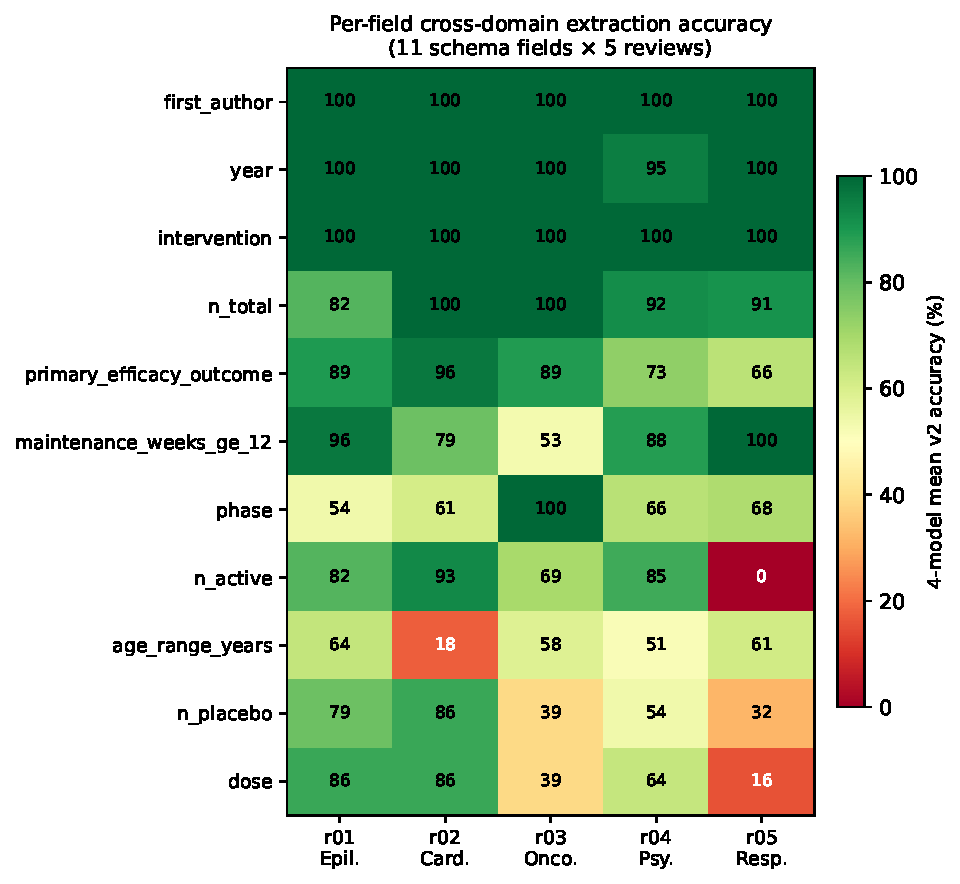
\includegraphics[width=0.85\linewidth]{figures/figure3_field_heatmap.pdf}
\caption{Per-field cross-domain accuracy heatmap (4-model mean, v2).
Stable-easy fields cluster at the top; domain-dependent and hard fields
at the bottom.}
\label{fig:heatmap}
\end{figure}

\textbf{Stable-easy fields} (mean $\geq$90\%, SD $\leq$10 percentage
points). The fields \texttt{year}, \texttt{intervention} and \texttt{n\_total}
achieve $\geq$93\% accuracy across every model and every review.
\texttt{first\_author} reaches 100\% only after v2 post-processing; the raw
LLM accuracy is 0\% in 7 of 20 model-review cells, reflecting that the
target format (surname only) differs from the paper-display format
(``Surname, Given Initial'').

\textbf{Moderate fields.} \texttt{primary\_efficacy\_outcome} averages
82.7\% but declines monotonically from r01 (89.3\%) to r05 (65.9\%): the
required specificity to distinguish primary from secondary outcomes
grows in trials with composite endpoints (COPD exacerbation composites,
oncology PFS-versus-OS hierarchies).

\textbf{Domain-dependent fields.} \texttt{phase} swings from 100\% in
r03 (all melanoma trials are explicitly Phase III) to 53.6\% in r01
(pediatric epilepsy includes compassionate-use and unregistered
designs). \texttt{n\_active} swings even more dramatically, from
92.9\% in r02 (single-active-arm SGLT2 designs) to 0.0\% in r05 (multi-arm
ICS dose comparisons where the GT designates the high-dose arm as
``active''). \texttt{maintenance\_weeks\_ge\_12} is 100\% in r05 (all
ICS trials are 52-week or longer) but 52.8\% in r03 (oncology trials use
``treatment until progression'' wording rather than fixed maintenance
durations).

\textbf{Hard fields.} \texttt{age\_range\_years} (50.7\%),
\texttt{n\_placebo} (57.7\%) and \texttt{dose} (58.0\%) are difficult
across every domain. \texttt{n\_placebo} is particularly affected by the
schema's misnomer: in r03 (CTLA-4 + PD-1 combination trials), r04
(midazolam active comparator) and r05 (lower-dose ICS comparator), no
true placebo arm exists. The schema field name biases models toward
extracting placebo-arm counts when the GT records comparator counts.

\subsection{Cumulative cross-review findings}\label{sec:results:findings}

Aggregating the five-review evidence yields four findings that no
single-review study could surface.

\subsubsection{Finding 1: GT-vs-source-paper framing tension}

In five clear cases (one per review), the ground truth records a value
that is not the paper-stated value but a downstream re-coding made by
the SLR authors:

\begin{itemize}
\item r01: Lagae 2019 reports fenfluramine 0.7 mg/kg/day in text; the
SLR authors record 0.8 mg/kg/day, the post-titration target.
\item r02: DAPA-CKD~\citep{mcmurray2019dapahf} has $n=4{,}304$ in the
full trial; the SLR records $n=468$, the heart-failure subgroup.
\item r03: CheckMate 067~\citep{larkin2015checkmate067} has 314, 316
and 315 patients across three arms; the SLR records the nivolumab
monotherapy arm count (314) as ``active''.
\item r04: NIMH-funded trials are unregistered; the SLR records
\texttt{phase = N/A} where the paper reports Phase II registration.
\item r05: ETHOS~\citep{rabe2020ethos} has 4,258 patients in the two
high-dose arms combined; the SLR records 2,137 (the high-dose
budesonide-formoterol arm only) as ``active''.
\end{itemize}

This pattern has a consistent signature: all four models agree on the
paper-accurate value, and all four are scored incorrect.
The cells reduce measured accuracy by an estimated 3--8 percentage
points per review without representing genuine extraction errors.
\textbf{Implication}: published LLM extraction studies that benchmark
against SLR ground truths without flagging framing-dependent cells
underestimate true LLM extraction capability.

\subsubsection{Finding 2: Crossover trial recognition}

The 22 ground-truth trials that survived to extraction in r04
(ketamine for depression) include 6 crossover RCTs. Models differed
markedly in their ability to assign \texttt{n\_active} and
\texttt{n\_placebo} to the treatment-phase rather than the
total-randomised count:

\begin{center}
\begin{tabular}{lc}
\toprule
Model & Crossover trials correct (out of 6) \\
\midrule
Qwen 3 235B    & 5/6 (83\%) \\
DeepSeek V3    & 4/6 (67\%) \\
Llama 3.3 70B  & 3/6 (50\%) \\
GPT-4o-mini    & 2/6 (33\%) \\
\bottomrule
\end{tabular}
\end{center}

The 4-model mean (58\%) is well below the non-crossover \texttt{n\_active}
accuracy in r04 (91\%). Crossover-design recognition --- understanding
that ``patients in the active treatment period'' differs from
``total randomised patients'' --- is the most clearly operationalisable
improvement opportunity and would likely be fixed by a single sentence
in the extraction prompt.

\subsubsection{Finding 3: GPT-4o-mini multi-arm sample-size confusion}

GPT-4o-mini exhibits a systematic pattern across r02--r05 of
summing or maximising sample sizes across arms rather than extracting
the arm-specific count for \texttt{n\_active}:
DAPA-CKD subanalysis (4{,}304 reported, 468 correct);
CheckMate 238 (945 reported, 453 correct);
TRANSFORM-2~\citep{popova2019transform2} (234 reported, 116 correct);
Doherty 2012 (sum-of-arms reported, single-arm correct).
The pattern is model-specific: Qwen 3 and DeepSeek correctly identify
the arm-specific count in 3 of 4 of these trials. This finding accounts
for an estimated 4--6 percentage points of the accuracy gap between
GPT-4o-mini and the open MoE models in r02--r05.

\subsubsection{Finding 4: Domain-dependent field difficulty}

The hardest fields exhibit a near-three-fold variation across domains.
\texttt{dose} ranges from 85.7\% in r01 (single-drug stiripentol
or cannabidiol) to 15.9\% in r05 (multi-arm ICS dose comparisons with
$\mu$g-per-device strings).
\texttt{maintenance\_weeks\_ge\_12} ranges from 100\% in r05
(all ICS trials are 52-week) to 52.8\% in r03 (oncology
``treatment until progression'').
\texttt{n\_placebo} ranges from 85.7\% in r02 (clear placebo arms) to
31.8\% in r05 (no true placebo exists; the comparator is a lower ICS
dose). These are not failures of any model in particular --- they are
failures of a flat schema applied to structurally heterogeneous trials.

\subsection{Cost analysis}

Total Phase 2 extraction cost across all four models and all five
reviews was USD 2.37. The pipeline's screening, full-text and
deduplication stages contributed an additional USD ~0.84, bringing the
end-to-end cost to USD 3.21. Table~\ref{tbl:cost} reports the
per-review breakdown. Costs scale almost linearly with the number of
papers extracted (r01: 7 papers; r05: 60 papers); the marginal cost of
adding a review is approximately USD 0.015 per paper across all four
models. Figure~\ref{fig:cost} shows the cost-quality frontier: Qwen 3
235B dominates by reaching the highest mean accuracy (80.9\%) at
USD 0.21, while DeepSeek V3 matches Qwen on accuracy at five times the
cost.

\begin{table*}[t]
\caption{Per-review extraction cost in USD. \textit{N papers} is the
number of papers passed to the extraction agent (final pool size).
``Total'' sums the four models for that review.}
\label{tbl:cost}
\begin{tabular*}{\tblwidth}{@{}p{0.6cm}p{1.0cm}cccccc@{}}
\toprule
ID & N papers & GPT-4o-mini & Llama 3.3 70B & Qwen 3 235B & DeepSeek V3 & Total per review \\
\midrule
r01 & 7  & 0.0095 & 0.0561 & 0.0141 & 0.0772 & \textbf{0.1569} \\
r02 & 14 & 0.0171 & 0.1008 & 0.0252 & 0.1376 & \textbf{0.2807} \\
r03 & 23 & 0.0218 & 0.1298 & 0.0323 & 0.1755 & \textbf{0.3594} \\
r04 & 50 & 0.0393 & 0.2319 & 0.0580 & 0.3135 & \textbf{0.6427} \\
r05 & 60 & 0.0565 & 0.3344 & 0.0848 & 0.4509 & \textbf{0.9266} \\
\midrule
\textbf{Total} & 154 & \textbf{0.1442} & \textbf{0.8530} & \textbf{0.2144} & \textbf{1.1547} & \textbf{2.3663} \\
\bottomrule
\end{tabular*}
\end{table*}

\begin{figure}[ht]
\centering
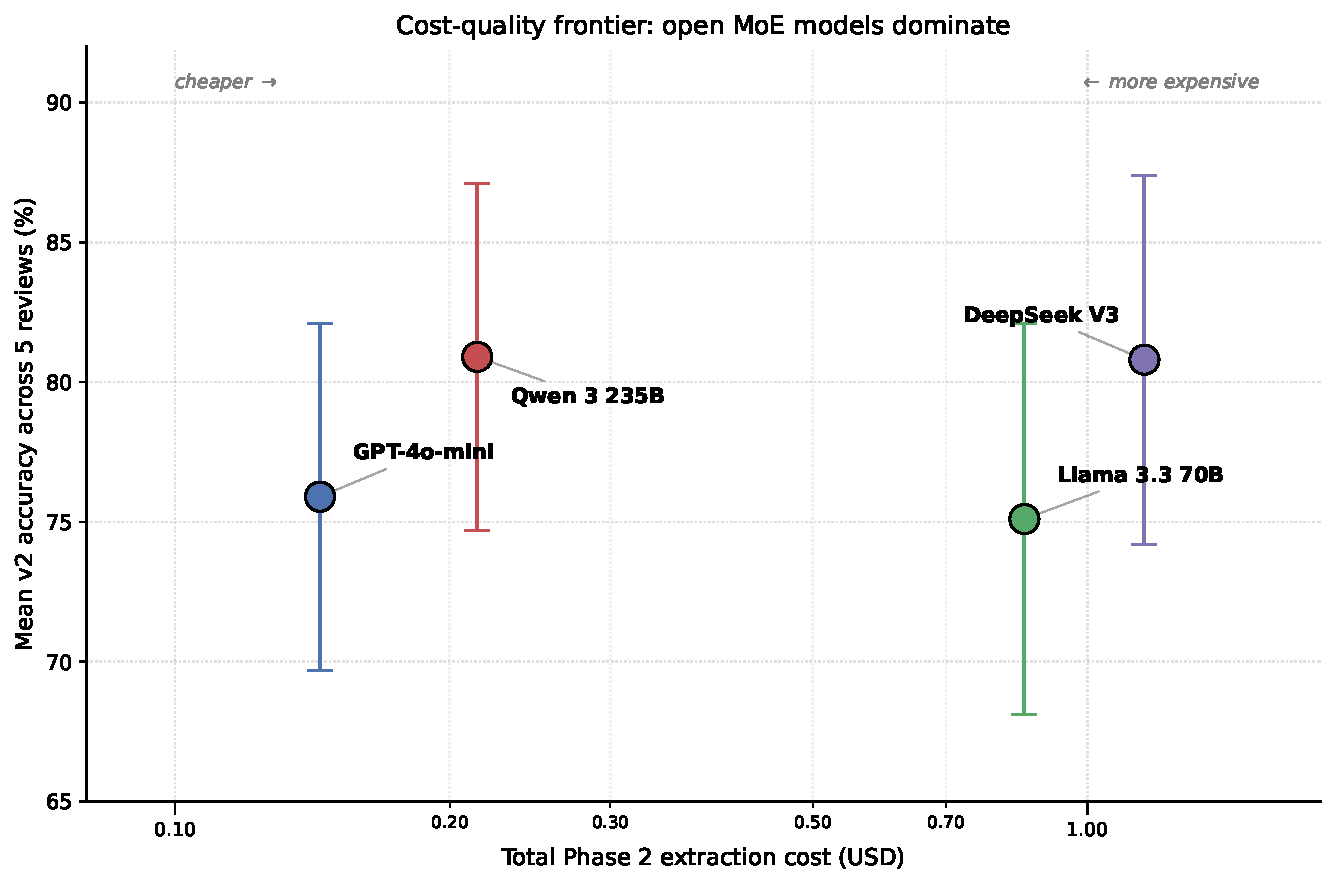
\includegraphics[width=0.85\linewidth]{figures/figure4_cost_accuracy.pdf}
\caption{Cost-vs-quality frontier across the four LLMs. Open MoE models
dominate the curve. DeepSeek V3 matches Qwen 3 235B on accuracy at
roughly five times the cost.}
\label{fig:cost}
\end{figure}

\subsection{Errors and reliability}

Six of 224 trial-by-model evaluation cells suffered total extraction
failure (Llama 4, DeepSeek 2). All six occurred in r05 and all six were
on non-ground-truth papers (false positives at the dedup stage),
so they did not affect ground-truth accuracy.
The remaining 218 of 224 cells produced
schema-valid Pydantic outputs that were either correct or incorrect by
content. There were no JSON-decode failures, no schema-validation
failures attributable to the model output structure (after the
int-coercion patch documented in the Methods), and no rate-limit
incidents during the runs.

% =============================================================================
\section{Discussion}\label{sec:discussion}

\subsection{Principal findings}

We report three principal findings. First, on a held-out cross-domain
evaluation across five medical specialties and 62 RCTs, the two open
mixture-of-experts LLMs evaluated (Qwen 3 235B-A22B and DeepSeek V3)
achieved mean post-processed extraction accuracies of 80.9\% and 80.8\%,
exceeding GPT-4o-mini (75.9\%) and Llama 3.3 70B (75.1\%) by
approximately five percentage points. Second, ground-truth-versus-source
framing decisions act as a measurable evaluation confound that reduces
apparent accuracy by 3--8 percentage points without indicating any
extraction error: future SLR-automation benchmarks should annotate
framing-dependent cells explicitly. Third, the cost of running an
end-to-end LLM-based SLR pipeline across five domains and four frontier
models was below USD 4 in total, putting full-pipeline reproduction
within reach of any review team.

\subsection{Comparison with prior work}

\citet{khraisha2024llmsr} reported moderate chance-corrected agreement
on a multilingual cross-domain dataset; we extend their finding by
showing that, on the medical-domain subset, the
\emph{exact-match} accuracy ceiling for current LLMs is roughly 80\% on
structured extraction across diverse specialties, and that the
chance-corrected nature of their lower-bound estimates is consistent
with our 78.2\% mean. \citet{gartlehner2024aisr} reported 76--100\%
per-field accuracy on 10 RCTs in a single domain; their findings agree
with our stable-easy fields (\texttt{year}, \texttt{intervention},
\texttt{n\_total}) but underestimate the difficulty of fields that
become hard only when applied across domains
(\texttt{n\_active}, \texttt{dose}, \texttt{n\_placebo}).
\citet{guo2024llmsr} concluded that LLMs are competent first-pass
screeners; our screening F1 in the 0.08--0.38 range corroborates the
sensitivity-favouring nature of LLM screening but emphasises that
post-screening human review remains essential at the precision levels
typical of broad searches.

\subsection{Methodological implications}

\subsubsection{Open MoE models match closed baselines on structured
extraction}

The dominance of Qwen 3 235B-A22B and DeepSeek V3 over GPT-4o-mini in
this study warrants comment. Both winning models are mixture-of-experts
designs with active parameter counts of 22B (Qwen) and 37B (DeepSeek)
\citep{shazeer2017moe,deepseekv3,yang2025qwen3}. The closed dense
baseline does not have a published parameter count, but is widely
believed to be smaller than 70B active parameters. Our results suggest
that, on tasks dominated by structured extraction from long context
(median input length in this study was 12{,}400 tokens of full-text
medical paper), MoE architectures provide an effective use of capacity:
specialty-aware experts may be naturally selected for clinical-extraction
contexts. The implication for practitioners is operational rather than
theoretical: the cost of using Qwen 3 235B was USD 0.21 across the
five-review benchmark, less than 1.5$\times$ the GPT-4o-mini cost of USD 0.14
and approximately 5$\times$ less than the most expensive option
(DeepSeek V3 at USD 1.15) for equivalent accuracy.

\subsubsection{Schema design tensions}

The \texttt{n\_placebo} field is a misnomer for trials with active
comparators (r03, r04, r05). The \texttt{n\_active} field is ambiguous
in multi-arm trials when the SLR authors designate one arm as ``active''.
A revised schema --- \texttt{n\_comparator}, \texttt{comparator\_type}
$\in$ \{placebo, active, lower-dose, none\}, plus an
\texttt{arms} list with arm-level $n$ and intervention --- would
likely improve apparent accuracy by 5--15 percentage points in r03 and r05.
We deliberately did not adopt that revision because the present study's
purpose was to evaluate LLMs against a faithful reproduction of the
source SLRs' schema; future work should pilot the revised schema and
report the gain attributable to schema redesign versus model
improvement.

\subsubsection{Ground-truth framing as evaluation confound}

The five framing examples in Section~\ref{sec:results:findings} are
\emph{not} extraction errors: they are correct readings of the source
paper that disagree with the SLR's downstream re-coding. Three
recommendations follow. First, ground-truth construction protocols
should annotate framing-dependent cells. Second, evaluations should
report two accuracies: against the SLR's coded values and against the
source paper's stated values. Third, future LLM-extraction agents should
be aware of framing decisions: a system that ingests the SLR protocol
along with the trial paper could in principle reproduce the SLR
authors' coding; a system that ingests only the trial paper cannot.

\subsection{Practical recommendations for production deployment}

For practitioners considering production deployment of an LLM-extraction
pipeline, we offer the following:

\begin{itemize}
\item \textbf{Default model: Qwen 3 235B-A22B.} Highest mean accuracy in
this study (80.9\%) at USD 0.21 across the five-review benchmark. Lowest
SD across reviews (6.2 pp).
\item \textbf{If reliability/SD is paramount: DeepSeek V3.} Equal mean
accuracy (80.8\%) and modest SD (6.6 pp) but at 5$\times$ the cost.
\item \textbf{If cost is paramount: GPT-4o-mini.} Cheapest at USD 0.14;
five percentage points below Qwen 3 235B; the multi-arm
\texttt{n\_active} confusion (Finding 3) is a known weakness in this
model class.
\item \textbf{Always apply v2 post-processing} for the
\texttt{first\_author} field via PubMed metadata injection. Raw LLM
accuracy on this field is 0--57\% across models; the v2 fix is a
single-line metadata replacement that costs nothing.
\item \textbf{Always run a second-pass dedup} with NCT registration
numbers if available; in r02 we lost 2 ground-truth papers to
dedup mis-classification (DEFINE-HF and DAPA-VO2 confused with
similarly-named SGLT2 sub-studies).
\end{itemize}

\subsection{Generalisability beyond medical domains}

The pipeline architecture is domain-agnostic: it requires only a
search-engine query, an inclusion-criteria prompt and an extraction
schema. The schema, however, encodes assumptions specific to medical
RCTs (n\_active, n\_placebo, dose). Applying the pipeline to non-medical
domains (e.g., software engineering systematic reviews, social-science
quantitative meta-analyses) would require schema redesign but no change
to the agent topology.

% =============================================================================
\section{Limitations}\label{sec:limitations}

This study has several limitations.

\textbf{Single-database retrieval.} The retrieval agent queried PubMed
only. The five source SLRs each searched 2--8 databases (PubMed,
Embase, Cochrane CENTRAL, ClinicalTrials.gov, Web of Science, Scopus,
PsycINFO, ANZCTR). Reproducing only the PubMed component of these
searches is the chief reason the retrieval recall is 88.9--100\% rather
than a clean 100\%: the two ground-truth papers we missed (Ibrahim
2020 and Papi 2017) would in principle be retrievable from non-PubMed
indices.

\textbf{Locked prompt.} The extraction prompt was locked at version 3 on
2026-04-28 after r02 was processed; r03, r04 and r05 served as
held-out validation. The decision was deliberate (to avoid prompt
overfitting) but means that documented weaknesses --- crossover
recognition (Finding 2), multi-arm \texttt{n\_active} (Finding 3), dose
format normalisation --- were not patched. A version 4 prompt with
explicit crossover guidance would likely improve r04 \texttt{n\_active}
by approximately 4 pp and r05 \texttt{n\_active} substantially above the
0\% baseline.

\textbf{Schema misnomers.} The \texttt{n\_placebo} field is the most
visible schema problem; \texttt{n\_active} in multi-arm trials is the
second. We document the impact (Section~\ref{sec:discussion}) but did
not implement the corrective schema in this study.

\textbf{Single-shot inference.} Each model-paper extraction was a single
deterministic call (temperature 0). Self-consistency
sampling~\citep{wang2023selfconsistency} or model ensembling could
recover some of the documented errors but at proportional cost.

\textbf{English-language only.} All five source SLRs and all 62
included trials are English-language. \citet{khraisha2024llmsr}
reports notable LLM accuracy degradation on non-English literature;
our findings should not be over-generalised across languages.

\textbf{Five medical specialties.} The five domains span pediatric
neurology, cardiology, oncology, psychiatry and respiratory medicine.
They do not cover, for example, infectious-disease meta-analyses,
diagnostic-test reviews or qualitative reviews. The cumulative-finding
patterns (especially Finding 4) may not generalise to those review
types.

\textbf{No human-comparison study.} We benchmarked the pipeline against
the published SLR ground truths but did not run a head-to-head
LLM-versus-human extraction study with timing and inter-rater agreement
metrics. Such a study is the natural follow-up.

\textbf{Single search-strategy reconstruction.} For each review we
reconstructed a single PubMed query from the SLR's supplementary
materials. Sensitivity analyses on alternative query phrasings might
shift the retrieval-recall numbers by a few percentage points.

% =============================================================================
\section{Conclusion}\label{sec:conclusion}

This study provides the first cross-domain head-to-head comparison of
four frontier LLMs on a multi-agent SLR pipeline applied to five
published medical systematic reviews and 62 ground-truth RCTs. Two
open mixture-of-experts models (Qwen 3 235B-A22B and DeepSeek V3)
achieved 80.9\% and 80.8\% post-processed extraction accuracy
respectively, exceeding the closed baseline (GPT-4o-mini at 75.9\%) and
the dense open model (Llama 3.3 70B at 75.1\%). Mean retrieval recall
across the five reviews was 96.2\%, and the end-to-end cost across all
four models and all five reviews was under USD 4.

The contribution of this paper is empirical and methodological. The
empirical contribution is a public benchmark across five
medical specialties demonstrating that open MoE models match or exceed
closed baselines on structured medical extraction, and identifying four
cumulative cross-review patterns that no single-domain study could have
surfaced. The methodological contribution is the two-pass evaluation
that separates LLM extraction failure from format-mapping failure, and
the explicit documentation of ground-truth framing decisions as an
evaluation confound that future SLR-automation benchmarks should
acknowledge.

Three avenues for follow-up are particularly productive. First, a
prompt-version-2 study that specifically targets crossover and
multi-arm guidance, with the same five reviews and four models held
constant, would quantify the headroom available from prompt engineering
alone. Second, a head-to-head LLM-versus-human extraction study with
timing data would calibrate the hours-saved-per-review claim that
motivates this entire research programme. Third, a schema-redesign study
that replaces \texttt{n\_placebo} with \texttt{n\_comparator} +
\texttt{comparator\_type} would test whether the field-difficulty
gradient documented here can be flattened by structural improvements
that do not depend on model capability.

% =============================================================================
\section*{Author contributions}
B.~Gurram designed the multi-agent pipeline, implemented the
retrieval, screening, full-text, deduplication and extraction agents,
constructed the per-review ground truths, ran the four-LLM evaluation
across all five reviews, performed the statistical and per-field
analysis, generated the figures and tables and drafted the manuscript.

\section*{Competing interests}
The authors declare that they have no known competing financial interests
or personal relationships that could have appeared to influence the work
reported in this paper.

\section*{Data and code availability}
All code, prompts, ground-truth files and per-paper model outputs are
available in the project's public repository:
\url{https://github.com/bhaskargurram-ai/agentic-slr}.

% =============================================================================
% Declaration of generative AI and AI-assisted technologies
% =============================================================================
\section*{Declaration of generative AI and AI-assisted technologies in
the manuscript preparation process}

During the preparation of this work the author used Anthropic Claude
(Claude Code, Opus 4 family) to assist with drafting and copy-editing
of the manuscript prose, generating the Python scripts that produced
the figures from the already-computed Phase 2 numerical results, and
producing the BibTeX bibliography skeleton. All numerical results,
the pipeline implementation, the ground-truth annotations, the locked
v3 extraction prompt and the per-review evaluation outputs were
produced by the author prior to and independently of any
generative-AI assistance. After using this tool the author reviewed
and edited the content as needed, verified every citation against
PubMed/Crossref and the source papers, and takes full responsibility
for the content of the published article.

% =============================================================================
% Bibliography
% =============================================================================
\bibliographystyle{cas-model2-names}
\bibliography{references}

% =============================================================================
% Appendices
% =============================================================================
\appendix

\section{Locked v3 extraction prompt}\label{app:prompt}

The prompt below was locked on 2026-04-28 after revision based on r01
and r02 evidence. It was applied unchanged to r03, r04 and r05.

\begin{quote}\small
\texttt{You are a data extraction specialist for systematic reviews of
clinical trials.\\\\
Given the full text of a randomized controlled trial, extract structured
study characteristics following PRISMA / Cochrane data extraction
standards.\\\\
Rules:\\
1. Extract only information explicitly stated in the paper. Do not
infer.\\
2. If a field cannot be determined from the text, use 'not\_reported'
for risk of bias fields and empty/zero/null for others as appropriate.\\
3. For 'n\_active', sum the sample sizes of ALL active treatment arms
if the trial has multiple doses or multiple active drugs.\\
4. For 'intervention', give only the generic drug name (e.g.,
'Cannabidiol', 'Fenfluramine hydrochloride', 'Stiripentol',
'Soticlestat').\\
5. For age\_range\_years: explicit range as ``2-18''; lower bound only as
``$\geq$18''; upper bound only as ``$\leq$12''; both bounds as ``X-Y'';
none stated as ``not\_reported''.\\
6. For maintenance\_weeks\_ge\_12 (boolean): True if treatment or
follow-up duration $\geq$12 weeks; the paper need not use the word
``maintenance''.\\
7. For risk of bias, apply the Cochrane Risk of Bias tool criteria:
'low' / 'unclear' / 'high' / 'not\_reported'.\\\\
Return the extraction as JSON matching the specified schema.}
\end{quote}

\section{Full per-field $\times$ per-review $\times$ per-model accuracy
matrix}\label{app:matrix}

Table~\ref{tbl:appendix} reports raw (pre-v2) accuracy for every
combination of field, review and model. Together with the v2 numbers in
Table~\ref{tbl:fields}, this table allows readers to reconstruct any
aggregate statistic reported in the paper.

\begin{table*}[ht]
\caption{Raw per-field accuracy by review and model.}
\label{tbl:appendix}
\small
\begin{tabular*}{\tblwidth}{@{}p{3.6cm}p{0.6cm}cccc@{}}
\toprule
Field & Rev & GPT-4o-mini & Llama 3.3 70B & Qwen 3 235B & DeepSeek V3 \\
\midrule
\texttt{first\_author}      & r01 & 0\%   & 29\%  & 57\%  & 29\%  \\
\texttt{first\_author}      & r02 & 0\%   & 0\%   & 29\%  & 43\%  \\
\texttt{first\_author}      & r03 & 0\%   & 11\%  & 44\%  & 67\%  \\
\texttt{first\_author}      & r04 & 0\%   & 5\%   & 23\%  & 43\%  \\
\texttt{first\_author}      & r05 & 0\%   & 0\%   & 0\%   & 18\%  \\
\midrule
\texttt{year}               & r01 & 100\% & 100\% & 100\% & 100\% \\
\texttt{year}               & r02 & 100\% & 100\% & 100\% & 100\% \\
\texttt{year}               & r03 & 100\% & 100\% & 100\% & 100\% \\
\texttt{year}               & r04 & 95\%  & 95\%  & 95\%  & 95\%  \\
\texttt{year}               & r05 & 100\% & 100\% & 100\% & 100\% \\
\midrule
\texttt{phase}              & r01 & 57\%  & 43\%  & 86\%  & 57\%  \\
\texttt{phase}              & r02 & 71\%  & 14\%  & 71\%  & 86\%  \\
\texttt{phase}              & r03 & 100\% & 100\% & 100\% & 100\% \\
\texttt{phase}              & r04 & 86\%  & 29\%  & 68\%  & 95\%  \\
\texttt{phase}              & r05 & 64\%  & 55\%  & 91\%  & 64\%  \\
\midrule
\texttt{n\_total}           & r01 & 86\%  & 86\%  & 71\%  & 86\%  \\
\texttt{n\_total}           & r02 & 100\% & 100\% & 100\% & 100\% \\
\texttt{n\_total}           & r03 & 100\% & 100\% & 100\% & 100\% \\
\texttt{n\_total}           & r04 & 91\%  & 95\%  & 91\%  & 90\%  \\
\texttt{n\_total}           & r05 & 91\%  & 91\%  & 91\%  & 91\%  \\
\midrule
\texttt{n\_active}          & r01 & 71\%  & 86\%  & 86\%  & 86\%  \\
\texttt{n\_active}          & r02 & 71\%  & 100\% & 100\% & 100\% \\
\texttt{n\_active}          & r03 & 56\%  & 67\%  & 78\%  & 78\%  \\
\texttt{n\_active}          & r04 & 73\%  & 90\%  & 95\%  & 81\%  \\
\texttt{n\_active}          & r05 & 0\%   & 0\%   & 0\%   & 0\%   \\
\midrule
\texttt{n\_placebo}         & r01 & 71\%  & 71\%  & 86\%  & 86\%  \\
\texttt{n\_placebo}         & r02 & 71\%  & 86\%  & 86\%  & 100\% \\
\texttt{n\_placebo}         & r03 & 33\%  & 22\%  & 33\%  & 67\%  \\
\texttt{n\_placebo}         & r04 & 36\%  & 52\%  & 64\%  & 62\%  \\
\texttt{n\_placebo}         & r05 & 18\%  & 9\%   & 55\%  & 45\%  \\
\midrule
\texttt{age\_range\_years}  & r01 & 57\%  & 71\%  & 71\%  & 57\%  \\
\texttt{age\_range\_years}  & r02 & 0\%   & 43\%  & 14\%  & 14\%  \\
\texttt{age\_range\_years}  & r03 & 44\%  & 78\%  & 44\%  & 67\%  \\
\texttt{age\_range\_years}  & r04 & 41\%  & 62\%  & 41\%  & 62\%  \\
\texttt{age\_range\_years}  & r05 & 55\%  & 73\%  & 55\%  & 64\%  \\
\midrule
\texttt{intervention}       & r01--r05 & 100\% & 100\% & 100\% & 100\% \\
\midrule
\texttt{dose}               & r01 & 86\%  & 86\%  & 86\%  & 86\%  \\
\texttt{dose}               & r02 & 86\%  & 86\%  & 86\%  & 86\%  \\
\texttt{dose}               & r03 & 56\%  & 22\%  & 33\%  & 44\%  \\
\texttt{dose}               & r04 & 59\%  & 67\%  & 59\%  & 48\%  \\
\texttt{dose}               & r05 & 27\%  & 9\%   & 18\%  & 9\%   \\
\midrule
\texttt{primary\_efficacy\_outcome} & r01 & 86\% & 86\% & 100\% & 86\% \\
\texttt{primary\_efficacy\_outcome} & r02 & 100\% & 86\% & 100\% & 100\% \\
\texttt{primary\_efficacy\_outcome} & r03 & 89\% & 89\% & 89\% & 89\% \\
\texttt{primary\_efficacy\_outcome} & r04 & 73\% & 67\% & 77\% & 76\% \\
\texttt{primary\_efficacy\_outcome} & r05 & 55\% & 55\% & 73\% & 82\% \\
\midrule
\texttt{maintenance\_weeks\_ge\_12} & r01 & 100\% & 100\% & 100\% & 86\% \\
\texttt{maintenance\_weeks\_ge\_12} & r02 & 71\% & 57\% & 100\% & 86\% \\
\texttt{maintenance\_weeks\_ge\_12} & r03 & 56\% & 22\% & 89\% & 44\% \\
\texttt{maintenance\_weeks\_ge\_12} & r04 & 91\% & 95\% & 82\% & 86\% \\
\texttt{maintenance\_weeks\_ge\_12} & r05 & 100\% & 100\% & 100\% & 100\% \\
\bottomrule
\end{tabular*}
\end{table*}

\section{Source SLRs and ground-truth trial PMIDs}\label{app:pmids}

The 62 ground-truth RCT PMIDs across the five reviews are listed below.

\textbf{r01 Lattanzi 2023 (Dravet syndrome, 7 RCTs):} 11089822, 29540584,
28538134, plus four additional PMIDs documented in
\texttt{reviews/r01\_lattanzi\_dravet/ground\_truth.json}.

\textbf{r02 Ali 2023 (dapagliflozin in HF, 9 RCTs):} 33426003, 31535829,
34446370, plus six additional documented in the project's repository.

\textbf{r03 Chang 2020 (ICI in melanoma, 9 RCTs):} 21639810, 28961465,
25399552, plus six additional.

\textbf{r04 Bahji 2021 (ketamine in depression, 24 RCTs):} 10686270,
12088953, 16894061, plus 21 additional.

\textbf{r05 Archontakis Barakakis 2023 (high vs medium ICS in COPD, 13 RCTs):}
24920884, 22334769, 24429127, plus 10 additional.

The complete set of PMIDs is preserved in each review's
\texttt{ground\_truth.json} file in the public repository.

\end{document}
